%!TEX root = ../VorlageBA.tex
\chapter{Grundlagen}

\section{Digital Imagery}
Digital imagery refers to visual content in digital form, that can be recognized and displayed by computers. For the purposes of this paper, we need to make a distinction between the following image types.

\begin{itemize}
	\item{Visible Spectrum(RGB) Imagery}
	\item{Thermal(Infrared) Imagery}
\end{itemize}

\subsection{Visible Spectrum(RGB) Imagery}

\cite{nasa_visiblelight} defines the visible light spectrum as the part of the electromagnetic spectrum visible to the human eye, ranging from approximately 380 to 700 nanometers in wavelength. This range encompasses all the colors perceivable by the human eye, from violet to red.

\subsection{Thermal(Infrared, IR) Imagery}
\cite{spi_thermal} defines thermal imaging, or thermography as the detection and measuring of radiation in the infrared spectrum being emitted from an object with the use of thermographic cameras. This type of imagery can collect temperature data from its field of view and display it using a variety of color palettes. Each pixel in a thermal image represents a temperature data point, and these data points are assigned a unique color or shade based on their value, meaning that as the thermal sensor detects changes in heat energy, it will express this change by adjusting the color or shade of a pixel. \citep{flir_colorpalette}

\begin{figure}[!ht]
	\centering
		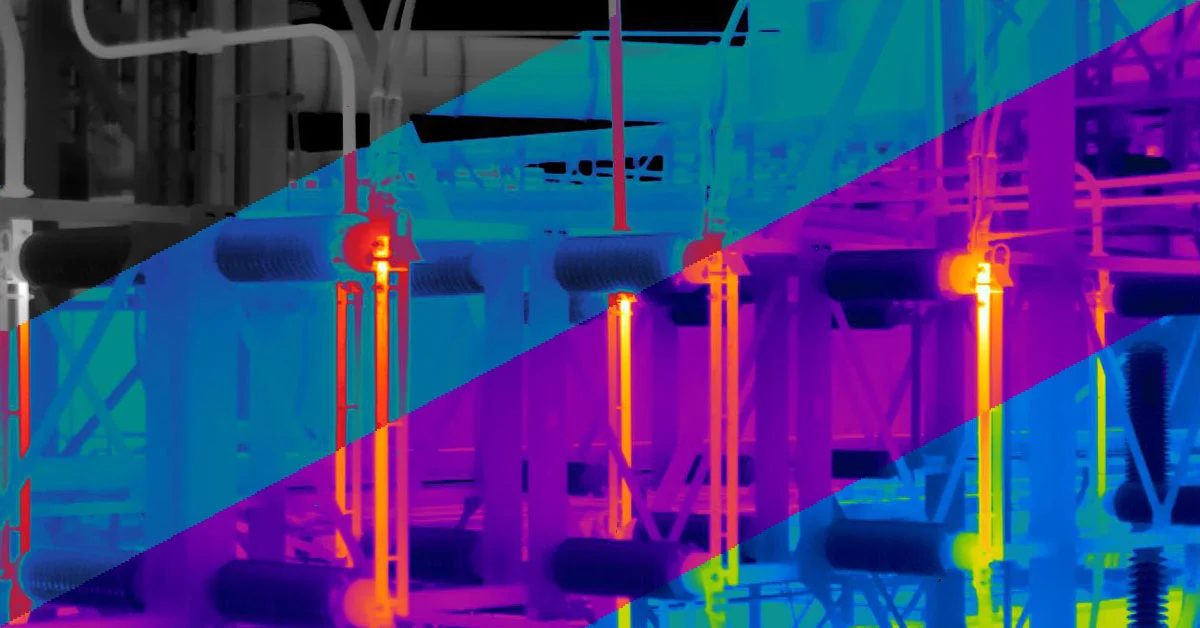
\includegraphics[width=0.75\textwidth]{images/color-palette-1200x628-fixed.png}
	\caption{Thermal Color Palettes \citep{flir_colorpalette}}
	\label{fig:color-palette}
\end{figure}

\section{Machine Learning (ML)}
\begin{quotation}
	\emph{``The studies reported here have been concerned with the
			programming of a digital computer to behave in a way
			which, if done by human beings or animals, would be
			described as involving the process of learning.''}
	\citep{samuel_machinelearning}
\end{quotation} 

Machine Learning is recognized to be a term originally coined by Arthur L. Samuel in \cite{samuel_machinelearning}. It refers to the behavior of a computer to learn by processing data, improving it's performance on certain tasks by working through a dataset and adjusting the algorithms to achieve better results. The idea is to require minimal human input while still performing well over a previously unseen set of data.

For a task to be fit for a machine learning application, a definite goal must exist, and at least one criterion or intermediate goal must exist which has a bearing on the achievement of the final goal and for which the sign should be known. \citep{samuel_machinelearning} Today, machine learning systems are used to identify objects in images, transcribe speech into text, match news items, posts or products with users’ interests, and select relevant results of search. \citep{deeplearning}

Machine learning algorithms essentially work by processing training data and refining certain parameters to increase performance. This happens through iterations on the data and adjusting parameters by increments. The types of machine learning can be defined as so:

\begin{description}
\item[Supervised Learning] is a very common method of machine learning, where the training data contains the expected output of an ML model. The training algorithm can then compute an objective function that measures the error (or distance) between the output scores and the desired pattern of scores \citep{deeplearning} and adjust the feature weights to improve the result by minimizing the error. The goal is to make correct predictions for new, unseen data.

\item[Unsupervised Learning] in contrast, does not contain any specific expected output within the training data. Thus the aim of the training is to recognize patterns within the dataset and categorize the data, rather than predicting an accurate label.

\item[Reinforcement Learning] algorithms that mimics how humans learn by trial and error. These algorithms use a reward and punishment paradigm, where the actions that work towards the goal are reinforcend and the actions that detract from the goal are punished or ignored. This feedback loop allows the algorithm to reach the goal by learning what is good and what is bad.

\end{description}


\subsection{Deep Learning}
A deep-learning architecture is a multilayer stack of simple modules, all (or most) of which are subject to learning, and many of which  compute non-linear input–output mappings. \citep{deeplearning} The multilayered structure allows automatic feature extraction from the data, which normally would need to be done manually and that often is a difficult task. Deep learning has the same fields of application as machine learning.

\subsection{Object Detection}

Object detection in digital images involves identifying and localizing objects within an image. This process not only recognizes the presence of objects but also depicts their precise boundaries, typically using bounding boxes. Unlike humans; computers can not easily identify objects inside an image and classify them as to what kind of object they are, whether that is an animal, a vehicle, a human or something else that such images could contain. 

Object detection in digital images has been its own field of study for a number of decades. The underlying algorithms for object detection have evolved significantly over the years, from traditional methods like sliding windows and handcrafted features to modern deep learning approaches. These deep learning models are trained on large datasets annotated with object classes and bounding boxes. During training, the network learns to minimize a loss function that penalizes incorrect classifications and inaccurate bounding boxes.

\subsection{Traditional Object Detection Methods}
\subsubsection*{Feature Selection by Hand}
Early object detection algorithms relied on features such as Haar-like features \citep{objdet_simplefeatures}, Scale-Invariant Feature Transform (SIFT) \citep{objdet_sift}, and Histogram of Oriented Gradients (HOG) \citep{objdet_hog}. These features are designed to capture relevant visual information about objects, which are then fed into classifiers like Support Vector Machines (SVMs) \citep{svm} or Decision Trees \citep{decisiontrees} to detect objects. However, these methods struggle with variations in object appearance and background clutter.

\subsubsection*{Sliding Window Approach}
One of the earliest techniques, this method involves moving a fixed-size window across the image and applying a classifier at each position to detect objects. Despite its simplicity, this approach is computationally intensive and often inefficient because it requires the classifier to be evaluated at every possible location and scale within the image. \cite{objdet_slidingwindow} utilizes the sliding window approach to object detection and classification for driver assistance systems.

\subsection{Modern Deep Learning Approaches to Object Detection}


\subsubsection{Convolutional Neural Networks (CNN)}
Convolutional Neural Networks' introduction to the object detection field has been revolutionary. CNNs are deep learning models that automatically learn feature representations from the data. CNN layers can progressively extract more complex features, from edges and boundaries in early layers to parts of objects and complete objects in the later layers.


\subsubsection{Region-Based Convolutional Neural Networks (R-CNN)} 
Region-Based Convolutional Neural Networks (R-CNN) have built upon the groundwork of CNNs by using selective search to propose regions likely to contain objects. Thus it reduces the number of locations to be checked. Each of these regions are then fed into a CNN. 

There are R-CNN variants that have further optimized this process to achieve better speed and accuracy such as Fast R-CNN \citep{girshick2015fast} and Faster R-CNN \citep{ren2016faster}

\subsubsection{You Only Look Once (YOLO)}
YOLO \citep{redmon2016look} models use a different approach by dividing the image into a grid and predicting bounding boxes and class probabilities directly for each grid cell in a single network pass. This architecture allows YOLO to achieve real-time object detection with greater speed. YOLO models may struggle with small or closely packed objects because of the way they are designed.

\subsubsection{Single Shot MultiBox Detector (SSD)}
Similar to YOLO, SSD predicts bounding boxes and class scores directly from feature maps. However, SSD uses multiple feature maps at different scales, allowing it to handle objects of various sizes more effectively.

%TODO Algorithms in detail


%TODO örnek tezleri incele benzer grundlagen çıkar


